\section{Warmte en Eerste Wet}
\subsection{Arbeid en Warmte}
Het is mogelijk de toestand van een systeem te veranderen zonder arbeid te verrichten. 

\begin{definition}
    \textbf{Adiabatische Arbeid}: Arbeid die wordt verricht zonder warmte-uitwisseling.
\end{definition}
\begin{definition}
    \textbf{Warmte}: Energie die wordt overgedragen tussen systemen als gevolg van een temperatuurverschil.
\end{definition}

Doordat een adiabatische wand geen warmte-uitwisseling toelaat, wordt deze een warmte-isolator genoemd. Een diathermische wand is een warmtegeleider.

\subsection{Inwendige Energie}

\begin{postulate}
    \textbf{Eerste Wet van de Thermodynamica}: De verandering in inwendige energie van een systeem is gelijk aan de som van de warmte die aan het systeem wordt toegevoegd en de arbeid die aan het systeem wordt verricht.
    \begin{equation}
        \Delta U = Q + W
    \end{equation}
    Waarbij:
    \begin{itemize}
        \item $\Delta U$ de verandering in inwendige energie is,
        \item $Q$ de warmte is die aan het systeem wordt toegevoegd (positief als het systeem warmte ontvangt, negatief als het warmte afgeeft),
        \item $W$ de arbeid is die aan het systeem wordt verricht (positief als er arbeid op het systeem wordt verricht, negatief als het systeem arbeid verricht).
    \end{itemize}   
\end{postulate}

\begin{definition}
    \textbf{Inwendige Energie functie}: De inwendige energie $U$ is een functie van de toestand van het systeem, en kan worden uitgedrukt als $U = U(S, V, N)$, waarbij $S$ de entropie is, $V$ het volume, en $N$ het aantal deeltjes.
    (Zie H9)
\end{definition}


\subsection{Wiskunde van de Eerste Wet}

De wiskundige formuleringg van de eerste wet hierboven bevat drie belanrijke ideëen:
\begin{itemize}
    \item De verandering in inwendige energie $\Delta U$ is een functie van de toestand van het systeem, en is dus een toestandsgrootheid. Het hangt alleen af van de begin- en eindtoestand van het systeem.
    \item Behoud energie
    \item Definitie van warmte als energieoverdracht als gevolg van een temperatuurverschil.
\end{itemize}
   

Een infinitesimaale hoeveelheid warmte \(\dbar Q\) kan niet worden uitgedrukt als differentiaal en is geen toestandsfunctie!

\begin{derivation}
    \textbf{Dubbelsysteem met adiabatische wand} dan geldt:
    \[ \Delta U_A = Q_A + W_A \] 
    en
    \[ \Delta U_B = Q_B + W_B \]
    \begin{align*}
        \implies \
        \Delta U_A + \Delta U_B &= (Q_A + Q_B) + (W_A + W_B)
    \end{align*}
        Omdat de wand adiabatisch is, is er geen warmte-uitwisseling tussen de systemen, dus \(Q_A + Q_B = 0\). Daarom kunnen we de vergelijking vereenvoudigen tot:
    \begin{align*}
        \Delta U_A + \Delta U_B &= W_A + W_B
    \end{align*}
    In adiabatische omstandigheden is de warmte verloren of gewonnen door het ene systeem gelijk aan de warmte gewonnen of verloren door het andere systeem.
    \qed
\end{derivation}


\subsection{Eerste Wet in Differentiaalvorm}

Voor een infinitesimale verandering in de toestand van het systeem kunnen we de eerste wet van de thermodynamica schrijven als:
\begin{equation}
    dU = \dbar Q + \dbar W
\end{equation}
Waarbij \(dU\) de differentiaal van de inwendige energie is, \(\dbar Q\) de infinitesimale hoeveelheid warmte is die aan het systeem wordt toegevoegd, en \(\dbar W\) de infinitesimale hoeveelheid arbeid is die aan het systeem wordt verricht.
Maar dit zou ondertussen niet meer hoeven uitgelegd te worden.

In ons hydrostatisch systeem:
\[
dU = \dbar Q - PdV
\]
In een dubbel hydrostatisch systeem:
\[
dU_A + dU_B = \dbar Q_A + \dbar Q_B - P_A dV_A - P_B dV_B
\]

De inwendige energie voor alle andere eerdere geziene systemen kunnen analoog bepaald worden:
\begin{itemize}
    \item Gespannen snaar: \(dU = \dbar Q + FdL\)
    \item Oppervlaktefilm: \(dU = \dbar Q + \gamma dA\)
    \item Elektrische cel: \(dU = \dbar Q + V_\epsilon dZ\) 
    
    (Hier gebruiken we \(Z\) voor de ladingen om dit niet te verwarren met de warmte \(Q\))
    \item Diëlektricum: \(dU = \dbar Q + E d\Pi\)
    \item Magnetisch systeem: \(dU = \dbar Q + \mu_0 H dM\)
\end{itemize}

Waarbij we analoog deze systemen kunnen combineren in een dubbel of zelf meervooudig systeem.

\begin{definition}
    \textbf{Pfaffiaanse differentiaalvormen}: De differentiaalvormen die voorkomen in de eerste wet van de thermodynamica, zoals \(dU\), \(\dbar Q\), en \(\dbar W\), worden Pfaffiaanse differentiaalvormen genoemd.
    Deze vormen zijn niet-exact, wat betekent dat ze niet kunnen worden uitgedrukt als de totale differentiaal van een functie van de toestand van het systeem.
    Als er maar twee verandelijken zijn, kan er wel steeds een integrerende factor worden gevonden, maar bij meer dan twee veranderlijken is dit niet altijd mogelijk. 
    Die integrerende factor zorgt ervoor dat de uitdrukking een totale differentiaal wordt, en dus een toestandsfunctie kan worden gedefinieerd.
\end{definition}


\subsection{Warmtecapaciteit}

\begin{definition}
    \textbf{Gemiddeldee Warmtecapaciteit}: 
    \[\bar{C} = \frac{Q}{T_f-T_i}\]
    Als Q en T infinitesimaal klein worden, kunnen we de gemiddelde warmtecapaciteit benaderen door de differentiaalvorm:
    \[C = \lim_{T_F \to T_i} \frac{Q}{T_f - T_i} =\frac{\dbar Q}{dT}\]
\end{definition}

\begin{definition}
    \textbf{Soortelijke Warmtecapaciteit}: De soortelijke warmtecapaciteit \(c\) is de warmtecapaciteit per eenheid massa van een stof, gedefinieerd als:
\[c = \frac{C}{m} = \frac{\dbar Q}{m dT}\]
Waarbij \(m\) de massa van de stof is.
\end{definition}

\begin{definition}
    \textbf{Molaire Warmtecapaciteit}: De molaire warmtecapaciteit \(C_m\) is de warmtecapaciteit per mol van een stof, gedefinieerd als:
\[C_m = \frac{C}{n} = \frac{1}{n}\frac{\dbar Q}{ dT}\]
Waarbij \(n\) het aantal mol van de stof is.
\end{definition}

\begin{definition}
    \textbf{Warmtecapaciteit bij constante druk}:
    \[C_P = \left( \frac{\dbar Q}{dT} \right)_P\]
\end{definition}

\begin{definition}
    \textbf{Warmtecapaciteit bij constant volume}:
    \[C_V = \left( \frac{\dbar Q}{dT} \right)_V\]
\end{definition}

We kunnen deze warmtecapaciteiten ook uitschrijven voor onze voorgaande systemen:
\begin{itemize}
    \item Hydrostatisch systeem: \(C_P = \left( \frac{\dbar Q}{dT} \right)_P\) en \(C_V = \left( \frac{\dbar Q}{dT} \right)_V\)
    \item Gespannen snaar: \(C_F = \left( \frac{\dbar Q}{dT} \right)_F\) en \(C_L = \left( \frac{\dbar Q}{dT} \right)_L\)
    \item Oppervlaktefilm: \(C_A = \left( \frac{\dbar Q}{dT} \right)_A\) en \(C_\gamma = \left( \frac{\dbar Q}{dT} \right)_\gamma\)
    \item Elektrische cel: \(C_{V_\epsilon} = \left( \frac{\dbar Q}{dT} \right)_{V_\epsilon}\) en \(C_Z = \left( \frac{\dbar Q}{dT} \right)_Z\)
    \item Diëlektricum: \(C_E = \left( \frac{\dbar Q}{dT} \right)_E\) en \(C_\Pi = \left( \frac{\dbar Q}{dT} \right)_\Pi\)
    \item Magnetisch systeem: \(C_H = \left( \frac{\dbar Q}{dT} \right)_H\) en \(C_M = \left( \frac{\dbar Q}{dT} \right)_M\)
\end{itemize}

\begin{definition}
    \textbf{Warmtereservoire}: Een warmtereservoire is een systeem met een zeer grote warmtecapaciteit, waardoor de temperatuur van het systeem bij het toevoegen of afvoeren van warmte vrijwel constant blijft.
\end{definition}

Voor een isobaar proces is de warmtecapaciteit:
\[C_P = \left( \frac{\dbar Q}{dT} \right)_P \implies Q_P = \int_{T_i}^{T_f} C_P dT = C_P (T_f - T_i)\]
Voor een isochor proces is de warmtecapaciteit:
\[C_V = \left( \frac{\dbar Q}{dT} \right)_V \implies Q_V = \int_{T_i}^{T_f} C_V dT = C_V (T_f - T_i)\]

Stel we kijken nu terug naar ons hydrostatisch systeem (\(\dbar Q = dU+PdV\)), dan kunnen we de warmtecapaciteit bij constante druk en constant volume ook uitdrukken in termen van \(U\):
\[U(T,V) \implies dU = \left( \frac{\partial U}{\partial T} \right)_V dT + \left( \frac{\partial U}{\partial V} \right)_T dV\]
\[U(P,T) \implies dU = \left( \frac{\partial U}{\partial P} \right)_T dP + \left( \frac{\partial U}{\partial T} \right)_P dT\]
\begin{align*}
    C_V &= \left( \frac{\dbar Q}{dT} \right)_V = \left( \frac{\partial U}{\partial T} \right)_V \\
    C_P &= \left( \frac{\dbar Q}{dT} \right)_P = \left( \frac{\partial U}{\partial T} \right)_P + P \left( \frac{\partial V}{\partial T} \right)_P
\end{align*}

\subsubsection{Inwendige energie van een gas}

Tijdens een \textbf{Vrije expansie} van een gas, waarbij het gas zich uitbreidt in een vacuüm zonder externe druk, is er geen arbeid verricht en geen warmte-uitwisseling (\(dU = dW = 0\)).
Dit impliceert dat de temperatuur oook niet verandert (\(dT = 0\)).

Gevolgen:
\[\left( \frac{\partial U}{\partial V} \right)_T = 0\]
\(U\) is volume onafhankelijk.
\[\left( \frac{\partial U}{\partial P} \right)_T = 0\]
Analoog is \(U\) druk onafhankelijk.

\subsubsection{Geval Ideaal Gas}

Voor eeen ideaal gas geldt:
\[PV = nRT\]
\textbf{Per definitie van een ideaal gas} geldt ook:
\[\left( \frac{\partial U}{\partial P} \right)_T = 0\]
Dit kan worden aangetoont in Hoofdstuk 9 door de iideale gaswet in de tweede energievergelijking te substitueren.

We kunnen:
\[\left( \frac{\partial U}{\partial P} \right)_T = \left( \frac{\partial U}{\partial V} \right)_T \left( \frac{\partial V}{\partial P} \right)_T  = 0\]
Met:
\[\left( \frac{\partial V}{\partial P} \right)_T = nRT\left( \frac{\partial \frac{1}{P}}{\partial P} \right)_T =-\frac{nRT}{P^2}\]
Ook herschrijven als:
\[\left( \frac{\partial U}{\partial P} \right)_T = -\frac{nRT}{P^2} \left( \frac{\partial U}{\partial V} \right)_T = 0 \implies \left(\frac{\partial U}{\partial V}\right)_T = 0\]

Hieruit leiden we af dat \(U = U(T)\) een functie is van de temperatuur alleen, en niet van het volume of de druk. Dit is een kenmerk van ideale gassen!

Uit \(C_V = \frac{dU}{dT}\) wordt de eerste hoofdwet voor een ideaal gas:
\begin{equation}
    \label{eq:1e-HW-C_V}
    \dbar Q = C_V dT + PdV
\end{equation}

De differentiatie van de ideale gaswet \(PV = nRT\) geeft:
\[PdV + VdP = nRdT\]
Hieruit kunnen we \(PdV\) vervangen in de eerste hoofdwet:
\[\dbar Q = C_V dT + nRdT - VdP = (C_V + nR) dT - VdP\]
\[\implies \frac{\dbar Q}{dT} = (C_V + nR) - V \left( \frac{dP}{dT} \right)\]
Hieruit kunnen we de warmtecapaciteit bij constante druk bepalen:
\[C_P  = \left( \frac{\dbar Q}{dT} \right)_P = C_V + nR \qquad  (P = cst)\]

Dit verteld ons twee beelangrijke zaken:
\begin{itemize}
    \item De warmtecapaciteit bij constante druk is altijd groter dan de warmtecapaciteit bij constant volume voor een ideaal gas \footnote{Omdat er bij constante druk ook arbeid wordt verricht door het gas tijdens de expansie}.
    \item De warmtecapaciteit bij constante druk en constant volume zijn beide functies van de temperatuur alleen!
\end{itemize}

Als we \(C_P = C_V + nR\) substitueren in \(\dbar Q = C_P dT - VdP\), krijgen we:
\begin{equation}
    \label{eq:1eHW-C_P}
     \dbar Q = C_P dT - VdP
\end{equation}


\subsection{Adiabastich Proces Ideaal Gas}
\begin{derivation}
    
Voor een adiabatisch proces geldt dat er geen warmte-uitwisseling is (\(\dbar Q = 0\)). We kunnen dit toepassen op de eerste hoofdwet voor een ideaal gas:
\[0 = C_V dT + PdV\]
en
\[0 = C_P dT - VdP\]

\[\implies \frac{dP}{P} = -\frac{C_P}{C_V} \frac{dV}{V} = -\gamma \frac{dV}{V}\]
Waarbij \(\gamma = \frac{C_P}{C_V}\) de adiabatische index is of ook de verhouding van de warmtecapaciteiten genoemd.
Integreren geeft:
\[
\int_{P_i}^{P_f} \frac{dP}{P} = -\gamma \int_{V_i}^{V_f} \frac{dV}{V}
\]
\[\implies \ln \left( \frac{P_f}{P_i} \right) = -\gamma \ln \left( \frac{V_f}{V_i} \right)  = \ln \left( \frac{V_i}{V_f} \right)^\gamma\]
\[\implies \frac{P_f}{P_i} = \left( \frac{V_i}{V_f} \right)^\gamma\]
\[\implies P_i V_i^\gamma = P_f V_f^\gamma\]
Of direct:
\[\ln P = -\gamma \ln V + \ln cst\]
\[\implies  PV^{\gamma} = cst\]
\qed
\end{derivation}

Voor monoatomische gassen is \(\gamma = \frac{5}{3} = cst\), voor diatomische gassen is \(\gamma = \frac{7}{5}\) en varieert ze een beetje met de temperatuur, en voor polyatomische gassen varieert \(\gamma\) 

Merk op dat in het geval van vrije epansie een adiabatisch proces niet quasistatisch verloopt.

We kunnen ook makkelijk met de ideale gaswet volgende relaties vinden:
\[ PV^\gamma = \frac{nRT}{V} V^\gamma = nRTV^{\gamma-1} = cst \]
In het adiabatisch proces stellen we dat het aantal deeltjes \(n\) constant is:
\[TV^{\gamma -1} = cst\]
Hieruit vinden we dan nog eens:
\[TV^{\gamma -1} = T \left( \frac{nRT}{V}\right)^{\gamma-1} = T^{\gamma}(nR)^{1-\gamma} V^{1-\gamma} = cst\]
Opnieuw is \(n = cst\) en \(R = cst\):
\[\implies T^{\gamma}V^{\gamma -1} = cst\]
\[\implies TP^{\frac{1-\gamma}{\gamma}} = cst\]
De Arbeid vericht in deze quasistische expansie van een ideaal gas wordt:
\begin{align*}
    W &= -\int_{V_i}^{V_f} PdV = -\int_{V_i}^{V_f} \frac{cst}{V^\gamma} dV = -cst \int_{V_i}^{V_f} V^{-\gamma} dV \\
    &= -\frac{cst}{1-\gamma} \left( V_f^{1-\gamma} - V_i^{1-\gamma} \right) = \frac{cst}{\gamma - 1} \left( V_f^{1-\gamma} - V_i^{1-\gamma} \right)
\end{align*}

Nu maken we gebruik van \(P_i V_i^\gamma = P_f V_f^\gamma = cst \):
\begin{align*}
    W &= \frac{1}{\gamma - 1} \left( P_f V_f^\gamma V_f^{1-\gamma} - P_i V_i^\gamma V_i^{1-\gamma} \right)\\
    &= \frac{1}{\gamma - 1} (P_f V_f - P_i V_i)
\end{align*}

Als de begin en eindtemperatuur bekend zijn, kunnen we dit sneller berekenen met \(PdV = -C_V dT\):
\begin{align*}
    W &= -\int_{V_i}^{V_f} PdV = \int_{T_i}^{T_f} C_V dT = C_V (T_f - T_i)
\end{align*}

\subsection{Experimentele data}

De warmtecapaciteit van vaste stoffen worden meestal bepaald aan de hand van de weerstand van een elektrische stroom,
waarbij de warmte die aan het systeem wordt toegevoegd kan worden berekend met \(Q = IVt \implies \dbar Q = I V_ dt\).
Voor metalen lijkt dit vrij logisch.

Om \(C_V \) van gassen te bepalen wordt vaak dezelfde methode toegepast, maar vaak iin een dunne metalen cilinder.
\(C_P\) wordt vaak bepaald met een doorstroomcaloriemeter.

\begin{derivation}
    Het bepalen van \(\gamma\) met de\textbf{methode van Rüchardt}:
    \begin{figure}[ht]
        \centering
        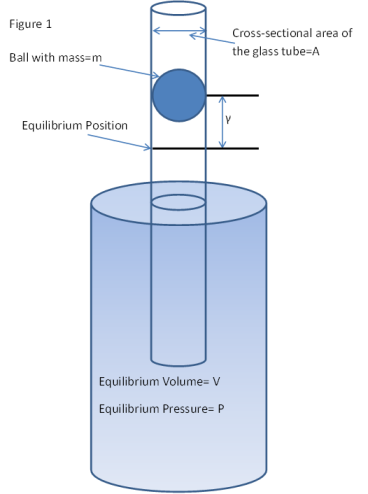
\includegraphics[width=0.5\linewidth]{Foto's-Figuren/Ruchard_experiment_layout.png}
        \caption{Schematische weergave van de methode van Rüchardt. \footnotesize \copyright{Wikipedia contributors} }
        \label{fig:Ruchard_experiment_layout}
    \end{figure}
    Een kogel met massa m wordt gebruikt als beweegbare zuiger. 
    De druk wanneer wrijving verwaarloosd wordt is:
    \[ P = P_{atm} + \frac{mg}{A} \]
    Waarbij \(A\) de oppervlakte van de kogel is. Deze oscilleert rond zijn evenwichtspositie,
    waarbij zich een klein volumeverandering plaatsvindt:
    \[\Delta V = Ay\]
    We kunnen de druk/kracht relatie \(F = A\Delta P\) gebruiken:
    \[\Delta P = \frac{F}{A}\]

    Als de kogel snel genoeg oscilleerd worden \(P\) en \(V\) als adiabatisch beschouwd een geldt \(PV^\gamma = cst\)
    of:
    \[P_\gamma V^{\gamma -1} \Delta V + V^\gamma \Delta P = 0\]
    Substitutie van \(\Delta V = Ay\) en \(\Delta P = \frac{F}{A}\) geeft:
    \[F = -\frac{\gamma PA^2 }{V}y \]

    De periode \(\tau\) wordt berekend door:
    \[\tau  = 2\pi \sqrt{\frac{m}{F}} = 2\pi \sqrt{\frac{mV}{\gamma PA^2}}\]
    Waaruit:
    \[\gamma = \frac{4\pi^2 mV}{\tau^2 PA^2}\]
    \qed
\end{derivation}
